\documentclass[11pt,a4paper]{article}
\usepackage[utf8]{inputenc}
\usepackage[T1]{fontenc}
\usepackage[spanish,es-nodecimaldot,es-tabla]{babel}
\usepackage{lmodern}
\usepackage[margin=2.3cm]{geometry}
\usepackage{amsmath,amssymb}
\usepackage{graphicx}
\usepackage{booktabs}
\usepackage{longtable}
\usepackage{float}
\usepackage{array}
\usepackage{caption}
\usepackage{enumitem}
\usepackage{xcolor}
\usepackage{multirow}
\usepackage[most]{tcolorbox}
\usepackage[hidelinks]{hyperref}
\usepackage{url}
\urlstyle{same}
\captionsetup{font=small,labelfont=bf}
\setlist{itemsep=1pt,topsep=3pt}
\sloppy
\newcommand{\Erms}{E_{\mathrm{rms}}}
\newcommand{\emx}{e_{\max}}
\newtcolorbox{caja}[1]{colback=gray!8,colframe=gray!60,title={#1},fonttitle=\bfseries,coltitle=black,colbacktitle=gray!20}

\title{\textbf{Reproducción de la curva tensión--estiramiento arterial con una base de materiales tipo fibra y una red neuronal}\\[4pt]\large Resumen del nivel del material para un trabajo interdisciplinario}
\author{Pablo Silvoni}
\date{24 de noviembre de 2026}
\begin{document}
\maketitle

\begin{abstract}
\noindent La pared arterial responde con una curva tensión--estiramiento en forma de J: blanda a bajo estiramiento y rígida a alto estiramiento. Este resumen presenta una herramienta para representar esa curva, la tensión circunferencial $\sigma_{\theta\theta}(\lambda_\theta)$, como suma de unos pocos materiales tipo fibra, cada uno con un número entero de láminas. Los materiales (la \emph{base}) se eligen una sola vez para toda una población, con tres criterios: precisión en las peores curvas, estabilidad numérica y cantidades no negativas. Para cada curva, el mejor diseño entero se calcula exactamente por programación lineal entera (diseño \emph{minimax}). Con esos diseños se entrena una red neuronal que, una vez entrenada, da las láminas de una curva nueva en una sola evaluación, sin optimizar. Con 41 carótidas humanas (Masson et al.) y 6 materiales, la red, con una revisión de $\pm1$ lámina, reproduce la curva con un peor error de 3\,\% del rango o menos en los 31 sujetos de entrenamiento, en los 10 de prueba y en 50 de 63 curvas de otros tres estudios; el minimax, que es el techo de lo alcanzable con láminas enteras, en 57 de esas 63.
\end{abstract}

%=====================================================================
\section{Qué se busca}
Un injerto vascular que se distiende distinto que la arteria que reemplaza altera el flujo cerca de las anastomosis y favorece la trombosis y la hiperplasia de la íntima~\cite{ding}. Los diseños publicados ajustan un solo número, la compliancia de una arteria promedio~\cite{harrison,tamimi,rovas23}. Pero la respuesta de una arteria no es un número: es una curva en J que cambia de un paciente a otro~\cite{holzapfel,humphrey}.

El objetivo de este nivel es \textbf{confeccionar la curva en J de cada arteria a partir de una base de materiales elegida de antemano}. Cada material es una fibra idealizada; la curva del injerto es la suma de los aportes de sus láminas; y lo que se elige para cada paciente es solo cuántas láminas lleva cada material. La herramienta final es una red neuronal entrenada dentro de un rango de curvas: recibe una curva $\sigma_{\theta\theta}(\lambda_\theta)$ y devuelve, en una evaluación, ese número de láminas.

Se trabaja con la curva tensión--estiramiento porque es una propiedad del tejido: no depende de la presión, del radio ni del espesor de la pared. Así, el método puede validarse con soluciones exactas antes de pasar a la geometría de un tubo.

\begin{caja}{Para el lector de elementos finitos}
La red neuronal cumple aquí el papel de un \emph{modelo sustituto} entrenado con soluciones ya calculadas. La etapa costosa se hace una vez, fuera de línea: elegir la base y resolver, para decenas de miles de curvas, el problema de optimización entera. La red aprende la relación entre la curva y su solución, y después la reproduce al instante, en línea, para una curva nueva. A diferencia de un modelo de orden reducido, no aproxima un campo: aproxima la \emph{solución de un problema de optimización}.
\end{caja}

%=====================================================================
\section{Datos: 41 carótidas y la franja de la población}
Masson et al.~\cite{masson} midieron en forma no invasiva el diámetro y la presión de la carótida común de 16 sujetos normotensos y 25 hipertensos tratados, y ajustaron a cada uno un modelo de la pared con elastina, cuatro familias de fibras de colágeno y tono muscular (14 parámetros por sujeto). Con esos parámetros se calcula, para cada sujeto, la tensión circunferencial en el borde media--adventicia en 999 valores de $\lambda_\theta$ entre 1,02 y 1,16. Las 41 curvas son J (monótonas y convexas) y van de 4,7 a 49\,kPa al comienzo y de 54 a 290\,kPa al final (Fig.~\ref{fig:sigma}). Diez sujetos (4 normotensos y 6 hipertensos) se reservan para prueba y no intervienen en ninguna elección del método.

Dos curvas límite, $y_1$ e $y_2$, encierran a los 41 sujetos. Esa franja es el \textbf{dominio de validez} de la herramienta: dentro de ella se generan las curvas de trabajo y de entrenamiento, y solo dentro de ella se garantiza el resultado de la red.

\begin{figure}[tb]\centering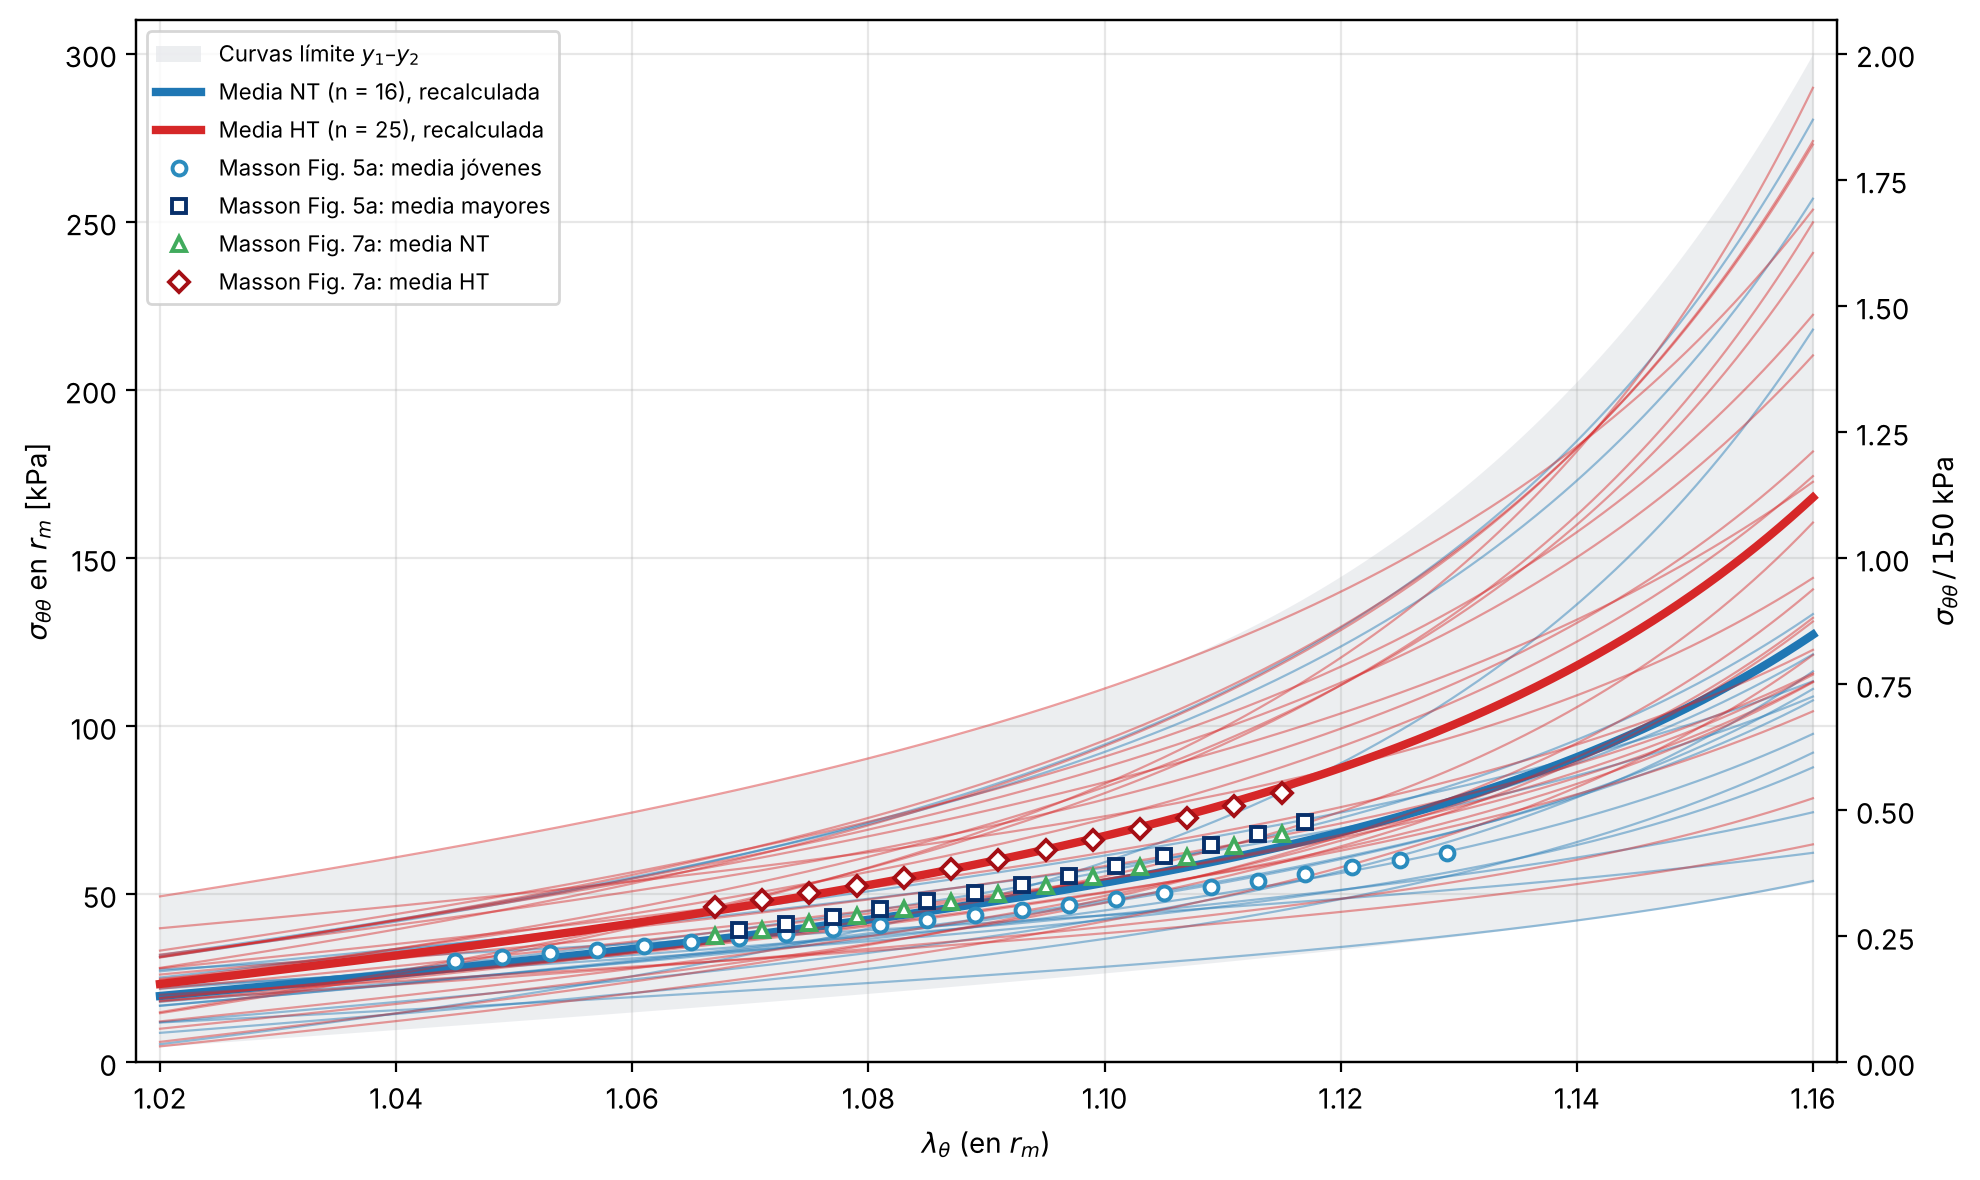
\includegraphics[width=0.74\textwidth]{fig1_sujetos_sigma_v49.png}
\caption{Los 41 sujetos de Masson et al.: tensión circunferencial en el borde media--adventicia (eje izquierdo en kPa; eje derecho, relativo a 150\,kPa). Franja gris: curvas límite $y_1$--$y_2$, el dominio de validez. Azul: normotensos; rojo: hipertensos.}\label{fig:sigma}\end{figure}

%=====================================================================
\section{La base de materiales}
\subsection{Un material es una recta truncada}
Una lámina del material $j$ aporta
\begin{equation}\label{eq:base}
A_j(\lambda)=S_j\,\max(0,\ \lambda-k_j):
\end{equation}
nada hasta su \emph{nudo} $k_j$, y desde ahí una recta de pendiente $S_j$. Es la idealización de una fibra rizada, que no tira hasta que el estiramiento la endereza; así se recluta el colágeno de la pared. La curva del injerto es la suma de los aportes de sus láminas,
\begin{equation}\label{eq:injerto}
\sigma_{\mathrm{inj}}(\lambda)=\sum_{j=1}^{N}z_j\,A_j(\lambda)=(Az)(\lambda),
\end{equation}
con $z_j$ el número de láminas del material $j$ y $A$ la matriz de la base (999 filas, una por valor de $\lambda$; $N$ columnas, una por material). Cada nudo produce un quiebre que hace la curva más empinada; con pocos nudos bien ubicados, la suma arma la J. Para nudos fijos, la curva del injerto es \textbf{lineal} en las láminas.

\subsection{Cómo se eligen los nudos}
Los nudos se eligen \textbf{una sola vez, para toda la población}, minimizando una función de costo $\Phi(k)$ evaluada sobre 22\,500 curvas sintéticas dentro de la franja y sobre los 31 sujetos de entrenamiento. $\Phi$ reúne tres exigencias:
\begin{itemize}
\item \textbf{Precisión en las peores curvas.} Para cada curva se calcula el peor error del ajuste por mínimos cuadrados. Se minimiza el CVaR 99\,\%~\cite{rockafellar}, el promedio de ese error sobre el 1\,\% de las curvas con mayor error. El promedio de todas dejaría sin control a las peores; la peor sola haría depender la elección de una única curva.
\item \textbf{Estabilidad numérica.} El número de condición de la base, $\kappa(A)=s_{\max}/s_{\min}$~\cite{trefethen}, acota cuánto se amplifica en las láminas un error relativo de la curva. Si dos nudos están muy juntos, sus columnas se parecen y el diseño se vuelve inestable: cantidades grandes de signo opuesto que se compensan. Se exige $\kappa(A)<30$.
\item \textbf{Cantidades fabricables.} Ninguna curva del dominio puede necesitar una cantidad negativa de un material, porque no se fabrica.
\end{itemize}
$\Phi$ no es derivable (un máximo, una ordenación y penalizaciones), por lo que se minimiza con un método global sin derivadas, la evolución diferencial~\cite{storn}, refinado con Nelder--Mead~\cite{nelder}. Dos restricciones físicas completan la elección:
\begin{itemize}
\item \textbf{El primer nudo va antes del dominio} ($k_1=0{,}82$). En $\lambda_\theta=1{,}02$ todas las arterias ya tienen tensión, y solo puede aportarla un material que ya esté trabajando. Ese material hace el papel de la elastina; se monta preestirado.
\item \textbf{La pendiente fija el tamaño de la lámina}: $S_j$ se elige para que ninguna curva del dominio necesite más de 20 láminas de un material.
\end{itemize}

\begin{figure}[tb]\centering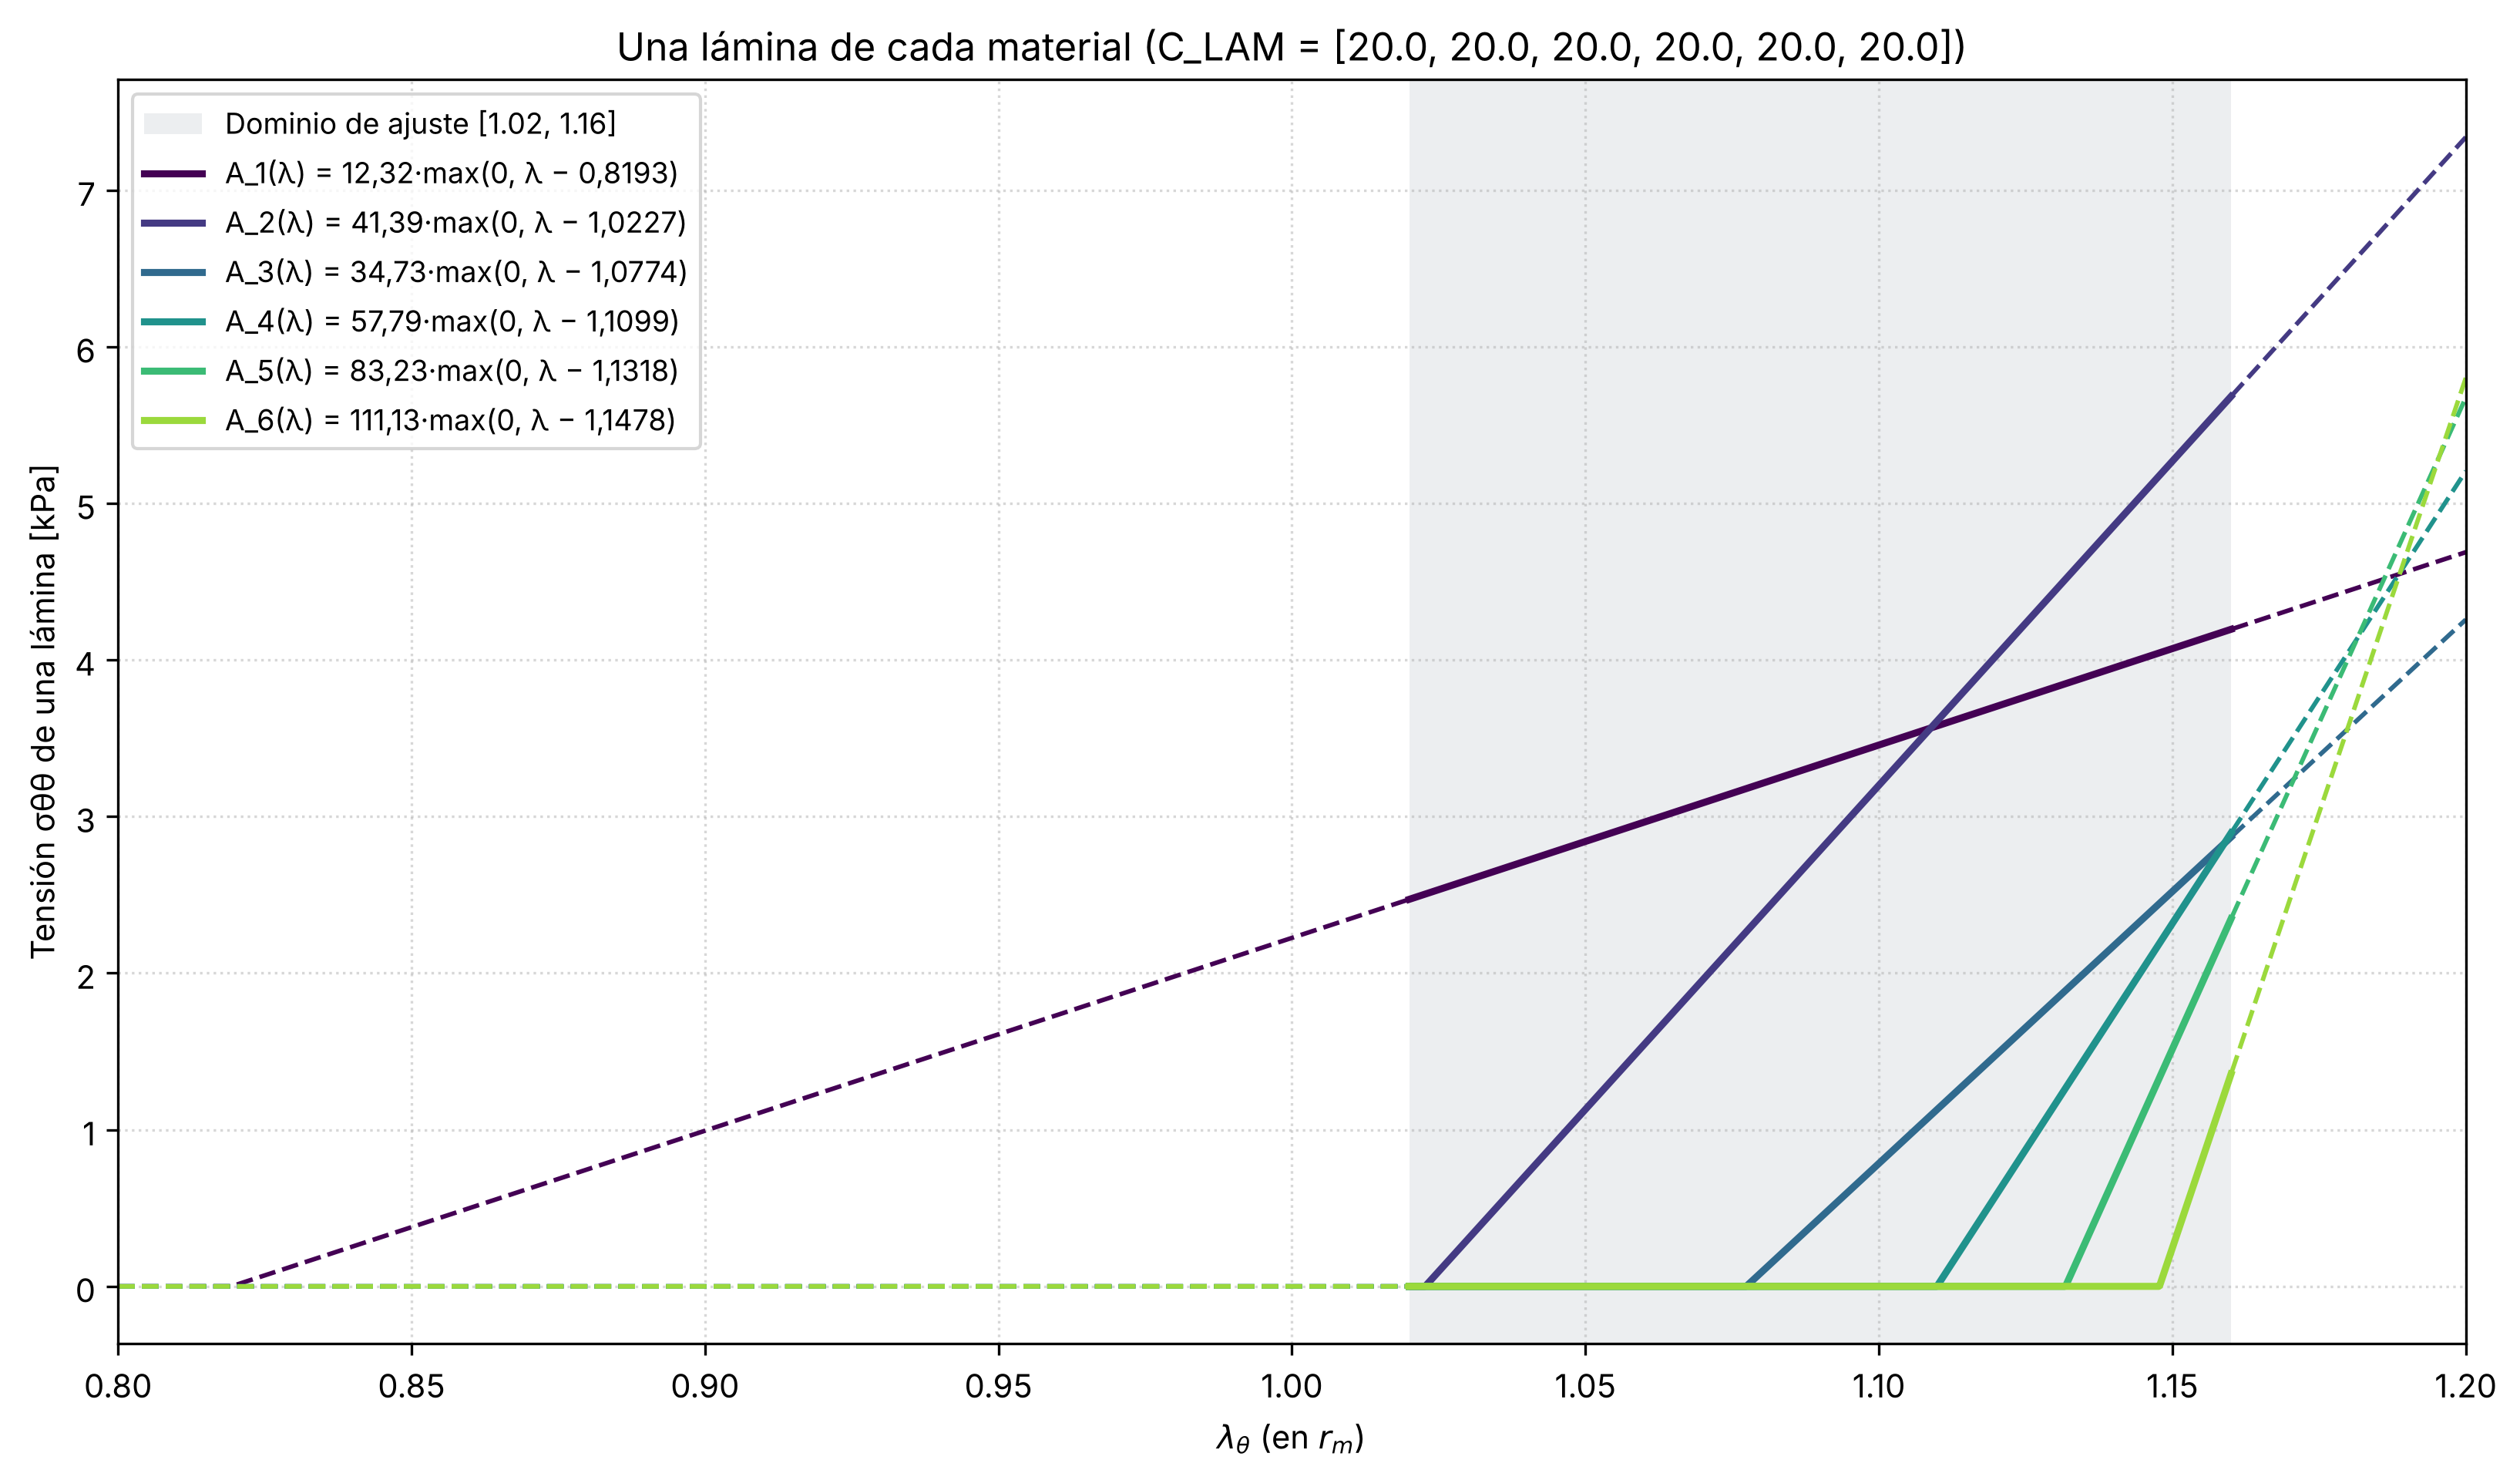
\includegraphics[width=0.6\textwidth]{bases_funcionales_v39_6.png}
\caption{La base de 6 materiales: una lámina de cada uno. El primer nudo está antes del dominio, como la elastina; los demás se agrupan donde la curva arterial se curva más.}\label{fig:bases}\end{figure}

\begin{table}[tb]\centering\small
\caption{Bases adoptadas: nudos $k_j$ y pendiente de una lámina $S_j$ [kPa]. Número de condición: 28,0 (6 materiales) y 19,0 (5).}\label{tab:bases}
\begin{tabular}{lcccccc}\toprule
 & 1 & 2 & 3 & 4 & 5 & 6\\\midrule
6 materiales, $k_j$ & 0,8193 & 1,0227 & 1,0774 & 1,1099 & 1,1318 & 1,1478\\
\phantom{6 materiales, }$S_j$ & 12,32 & 41,39 & 34,73 & 57,79 & 83,23 & 111,13\\\addlinespace
5 materiales, $k_j$ & 0,8228 & 1,0243 & 1,0881 & 1,1226 & 1,1447 & ---\\
\phantom{5 materiales, }$S_j$ & 12,56 & 43,57 & 51,92 & 88,74 & 129,08 & ---\\\bottomrule
\end{tabular}
\end{table}

\textbf{La base alcanza.} Con cantidades reales (mínimos cuadrados, $z=A^+y$~\cite{penrose,golub}), los 41 sujetos y todas las curvas del dominio quedan dentro de la meta, con un peor error de 0,88\,\% (6 materiales) y 1,41\,\% (5).

%=====================================================================
\section{De cantidades reales a láminas enteras: el diseño minimax}
\subsection{La métrica}
Para una curva objetivo $y$ con rango $\Delta=\max y-\min y$ y una curva de injerto $\hat y$,
\begin{equation}\label{eq:emax}
e_{\max}=\frac{100}{\Delta}\max_i\,\lvert y_i-\hat y_i\rvert\quad[\%].
\end{equation}
Es el peor punto, en porcentaje del rango: el criterio es igual de exigente con una arteria blanda que con una rígida. \textbf{Meta: $e_{\max}\le3$\,\%.} Todo diseño se compara con la curva original.

\subsection{Por qué minimax}
Un injerto se fabrica con láminas enteras, de 0 a 20 por material. Redondear la solución real de mínimos cuadrados no da en general el mejor diseño entero: al redondear seis cantidades, los errores pueden sumarse en un mismo tramo de la curva. Por eso se buscan directamente los enteros que dejan el ``túnel'' más angosto alrededor de la curva,
\begin{equation}\label{eq:minimax}
\min_{z,\tau}\ \tau\quad\text{sujeto a}\quad -\tau\le\frac{100}{\Delta}\bigl(y_i-(Az)_i\bigr)\le\tau\ \ (i=1,\ldots,999),\qquad z_j\in\{0,1,\ldots,20\}.
\end{equation}
Es una aproximación de Chebyshev~\cite{cheney} con variables enteras: un programa lineal entero mixto, que se resuelve por ramificación y acotación con HiGHS~\cite{highs} en unos 50 a 65\,ms por curva. Se usa por tres razones:
\begin{enumerate}[label=(\roman*)]
\item \textbf{Mide lo que importa.} Minimiza el peor punto, que es la meta del diseño. Un criterio cuadrático podría esconder un tramo mal copiado entre muchos puntos buenos.
\item \textbf{Da el óptimo global.} Es el diseño entero de menor $e_{\max}$ que existe. Si el minimax no cumple la meta en una curva, ninguna combinación de láminas la cumple. Por eso es la referencia contra la que se juzga la red.
\item \textbf{Da etiquetas exactas para entrenar.} Para cada curva de entrenamiento, la respuesta correcta que la red debe aprender está definida sin ambigüedad: es la solución de~\eqref{eq:minimax}.
\end{enumerate}
Con 6 materiales, el minimax cumple la meta en los 41 sujetos (peor 2,34\,\%).

%=====================================================================
\section{La red neuronal}
\subsection{Qué es y qué hace aquí}
Una red neuronal es una función con muchos parámetros, compuesta por capas: cada capa multiplica su entrada por una matriz, le suma un vector y le aplica una función no lineal simple. Los parámetros se ajustan minimizando una medida de error sobre muchos ejemplos de entrada y salida conocidas, como una calibración por mínimos cuadrados pero con cientos de miles de parámetros. Con suficientes neuronas, una red así puede aproximar cualquier función continua en un conjunto acotado~\cite{cybenko,hornik}.

Aquí la entrada es la curva $\sigma_{\theta\theta}(\lambda_\theta)$ en sus 999 puntos y la salida son las láminas enteras de cada material. Los ejemplos son 34\,503 curvas dentro de la franja, cada una con su diseño minimax como respuesta correcta. Una vez entrenada, la red da el diseño de una curva nueva \textbf{sin resolver ninguna optimización}.

Entrenar una red con las soluciones óptimas de un problema entero para que proponga al instante la de un caso nuevo es un esquema establecido del aprendizaje automático para optimización combinatoria~\cite{bengiolodi,nair}. En mecánica arterial, en cambio, las redes se usan hasta ahora para \emph{identificar} el tejido: obtener sus parámetros~\cite{liuml,utrera} o su ley constitutiva~\cite{linka,vervenne}. Aquí la red \emph{diseña}.

\subsection{Arquitectura: la red en cadena con salida ordinal}
Dos ideas adaptan la red a este problema (Fig.~\ref{fig:cadena}).
\begin{itemize}
\item \textbf{Salida ordinal.} Las láminas son cantidades ordenadas: errar por una no es lo mismo que errar por diez. Por eso, para cada material, la red no elige una entre 21 opciones sin orden, sino que responde 20 preguntas: ``¿lleva más de $k$ láminas?'' ($k=0,\ldots,19$). El número de láminas es la cantidad de respuestas afirmativas~\cite{frankhall,lilin,cao}. Así, cuando la red se equivoca, lo hace por poco.
\item \textbf{Decisión en cadena.} Los materiales se compensan entre sí: una lámina de más en uno puede corregirse con una de menos en el siguiente. Por eso la red decide de a un material, y cada uno sabiendo lo que se eligió en los anteriores~\cite{read11,dembczynski}.
\end{itemize}
Un tronco común ($999\to256\to128\to64$) resume la curva en un vector $h$ de 64 números. La cabeza del material $j$ recibe $h$ y las láminas ya elegidas de los materiales $1,\ldots,j-1$, y responde sus 20 preguntas. Al entrenar, cada cabeza recibe las láminas del minimax de los materiales anteriores; al usarla, las que eligió la propia red.

\begin{figure}[tb]\centering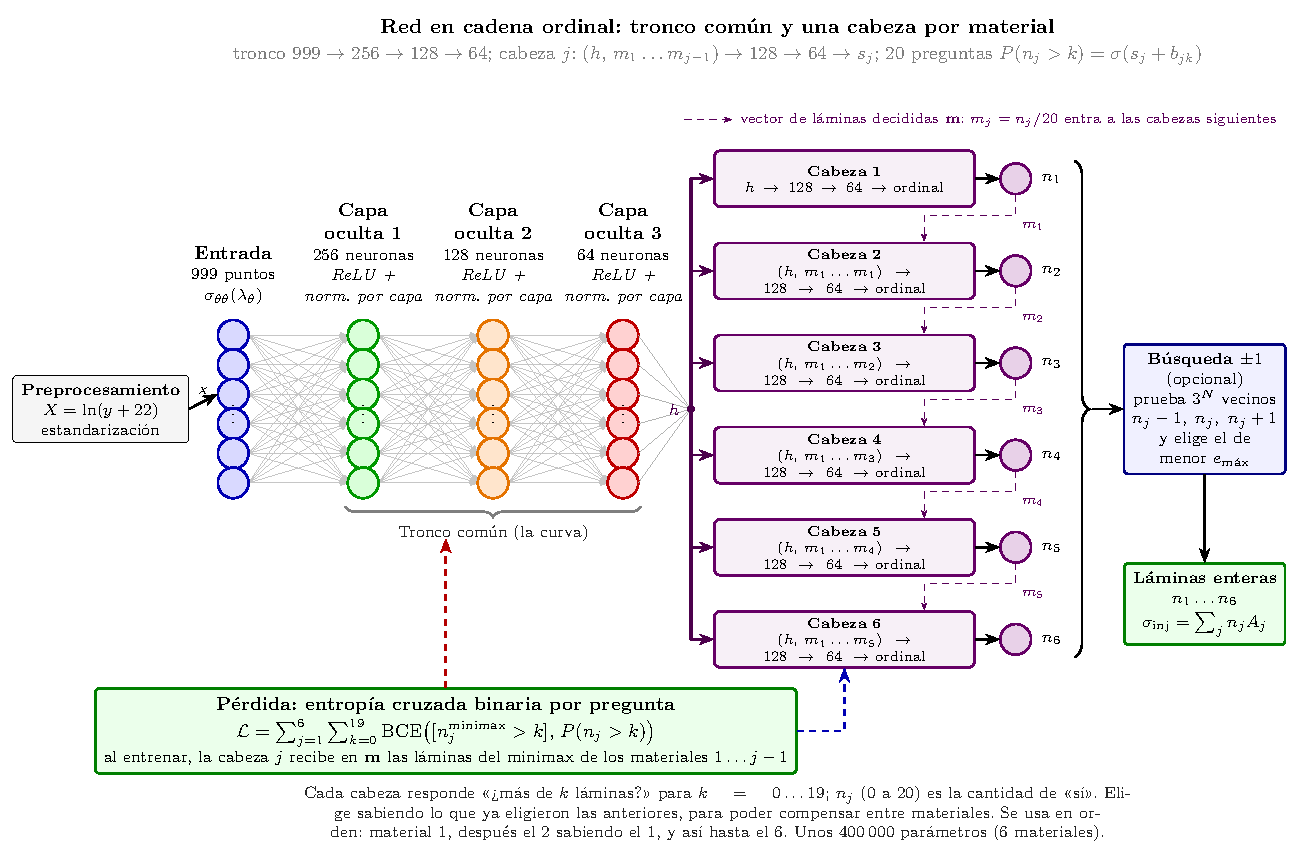
\includegraphics[width=0.95\textwidth]{red_cadena_es.pdf}
\caption{Red en cadena para 6 materiales. El tronco común resume la curva en $h$; la cabeza $j$ recibe $h$ y las láminas ya elegidas de los materiales anteriores ($m_i=n_i/20$) y responde las 20 preguntas ``¿más de $k$ láminas?''; $n_j$ es la cantidad de respuestas afirmativas. La búsqueda de $\pm1$, opcional, revisa las combinaciones vecinas de la respuesta.}\label{fig:cadena}
\end{figure}

\subsection{Entrenamiento}
Las curvas de entrenamiento son 50\,000, de siete familias: tres de la ley de Masson con parámetros de los sujetos de entrenamiento mezclados, perturbados o sorteados en su rango; otra ley exponencial; los 31 sujetos de entrenamiento; y dos familias de sumas de láminas de la propia base. Se conservan las 34\,503 que quedan dentro de la franja $y_1$--$y_2$, y se separan 24\,151 para entrenar, 3451 para validar y 6901 para probar. A cada curva se le agrega un ruido de 1\,\% al entrar a la red, y su respuesta correcta son sus láminas minimax. La pérdida es la entropía cruzada de las 20 preguntas de cada material, que equivale a maximizar la verosimilitud de las respuestas del minimax. El entrenamiento usa Adam~\cite{adam} y TensorFlow~\cite{tf}, y tarda unos 16 minutos de CPU.

\subsection{Revisión de $\pm1$ lámina}
A la respuesta de la red se le aplica, opcionalmente, una revisión: se evalúan las $3^N$ combinaciones que difieren en a lo sumo una lámina por material (729 con 6 materiales) y se elige la de menor $e_{\max}$. Es solo evaluar $Az$ en cada combinación, sin optimizar.

%=====================================================================
\section{Resultados}
La Tabla~\ref{tab:resumen} resume los resultados con 6 materiales, por separado para los sujetos que la red vio al entrenarse, los de prueba, 2000 curvas del dominio y 63 curvas de otros tres estudios.

\begin{table}[H]\centering\small
\caption{6 materiales, láminas enteras: $e_{\max}$ mediano / peor [\%] · curvas que cumplen la meta (3\,\%; 4\,\% en las 2000 curvas del dominio). Errores contra la curva original.}\label{tab:resumen}
\begin{tabular}{lccc}\toprule
Conjunto & Minimax (referencia) & Red en cadena & Red + revisión $\pm1$\\\midrule
Masson, entrenamiento (31) & 1,01 / 2,34 · 31 & 1,26 / 2,34 · 31 & 1,09 / 2,34 · 31\\
Masson, prueba (10) & 1,04 / 1,61 · 10 & 1,27 / 2,82 · 10 & 1,07 / 1,61 · 10\\
Curvas del dominio (2000) & 1,06 / 3,28 · 2000 & 1,22 / 4,93 · 1998 & 1,10 / 4,93 · 1999\\
Otros estudios (63) & 1,91 / 5,71 · 57 & 2,26 / 9,44 · 46 & 2,12 / 6,16 · 50\\\bottomrule
\end{tabular}
\end{table}

\begin{itemize}
\item \textbf{Sujetos de prueba.} La red cumple la meta en los 10, sola y con la revisión de $\pm1$; con la revisión, su peor caso es igual al del minimax (1,61\,\%).
\item \textbf{Otros estudios.} Sin cambiar nada (mismos nudos, misma red, misma franja), se aplicó a curvas de carótidas común, externa e interna recalculadas con las leyes y parámetros que publicaron sus autores: Sommer y Holzapfel~\cite{sommer} (ex vivo, pared intacta y media--íntima), Liu et al.~\cite{liu} y Kamenskiy et al.~\cite{kamenskiy} (in vivo). De 98 curvas, 63 quedan dentro de la franja. La red con revisión cumple en 50 y el minimax en 57; en las 6 restantes ningún diseño entero cumple. Son curvas in vivo casi rectas y de poco recorrido de tensión, en las que una sola lámina mueve la curva más de lo que permite la meta.
\item \textbf{Muchos diseños sirven.} La red da exactamente las láminas del minimax en pocos sujetos (6 de 41), pero donde difiere lo hace en una o dos láminas con errores parecidos: varias combinaciones enteras reproducen casi igual la misma curva. Por eso la red se juzga por el error de la curva y no por coincidir con el minimax.
\item \textbf{Tiempo.} El minimax tarda de 50 a 65\,ms por curva. La red, en lote, 0,3\,ms por curva, y con la revisión de $\pm1$, 2,0\,ms: de 30 a 200 veces menos.
\end{itemize}

\begin{figure}[tb]\centering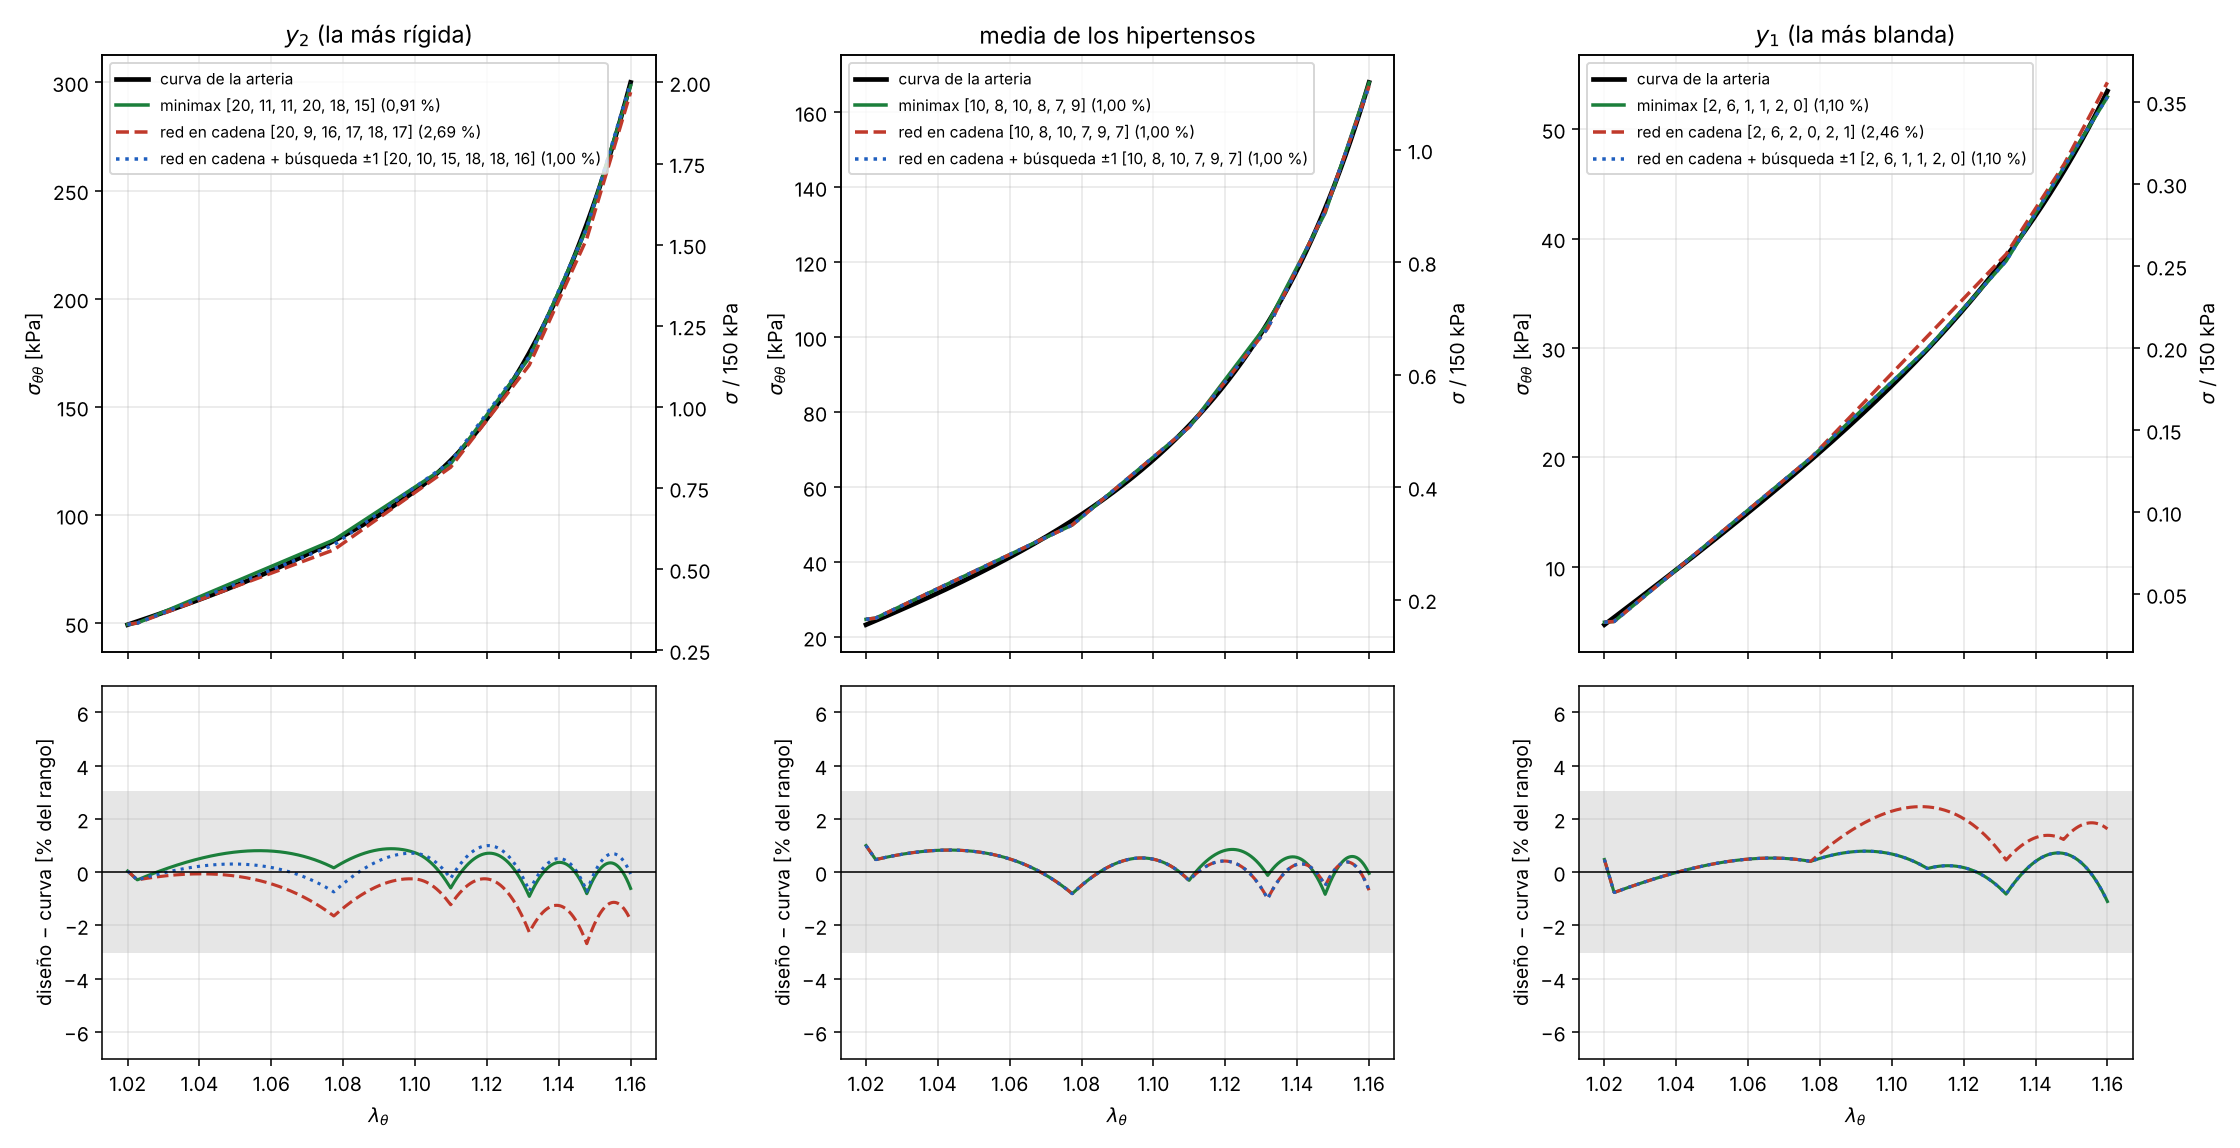
\includegraphics[width=0.9\textwidth]{v58_limite_es.png}
\caption{6 materiales: la curva más rígida de la franja ($y_2$), la media de los hipertensos y la más blanda ($y_1$). Arriba: tensión, con las láminas de cada material y el $e_{\max}$ de cada diseño; abajo: diseño $-$ curva en \% del rango (franja gris: meta de $\pm3$\,\%).}\label{fig:limite}\end{figure}

\begin{figure}[tb]\centering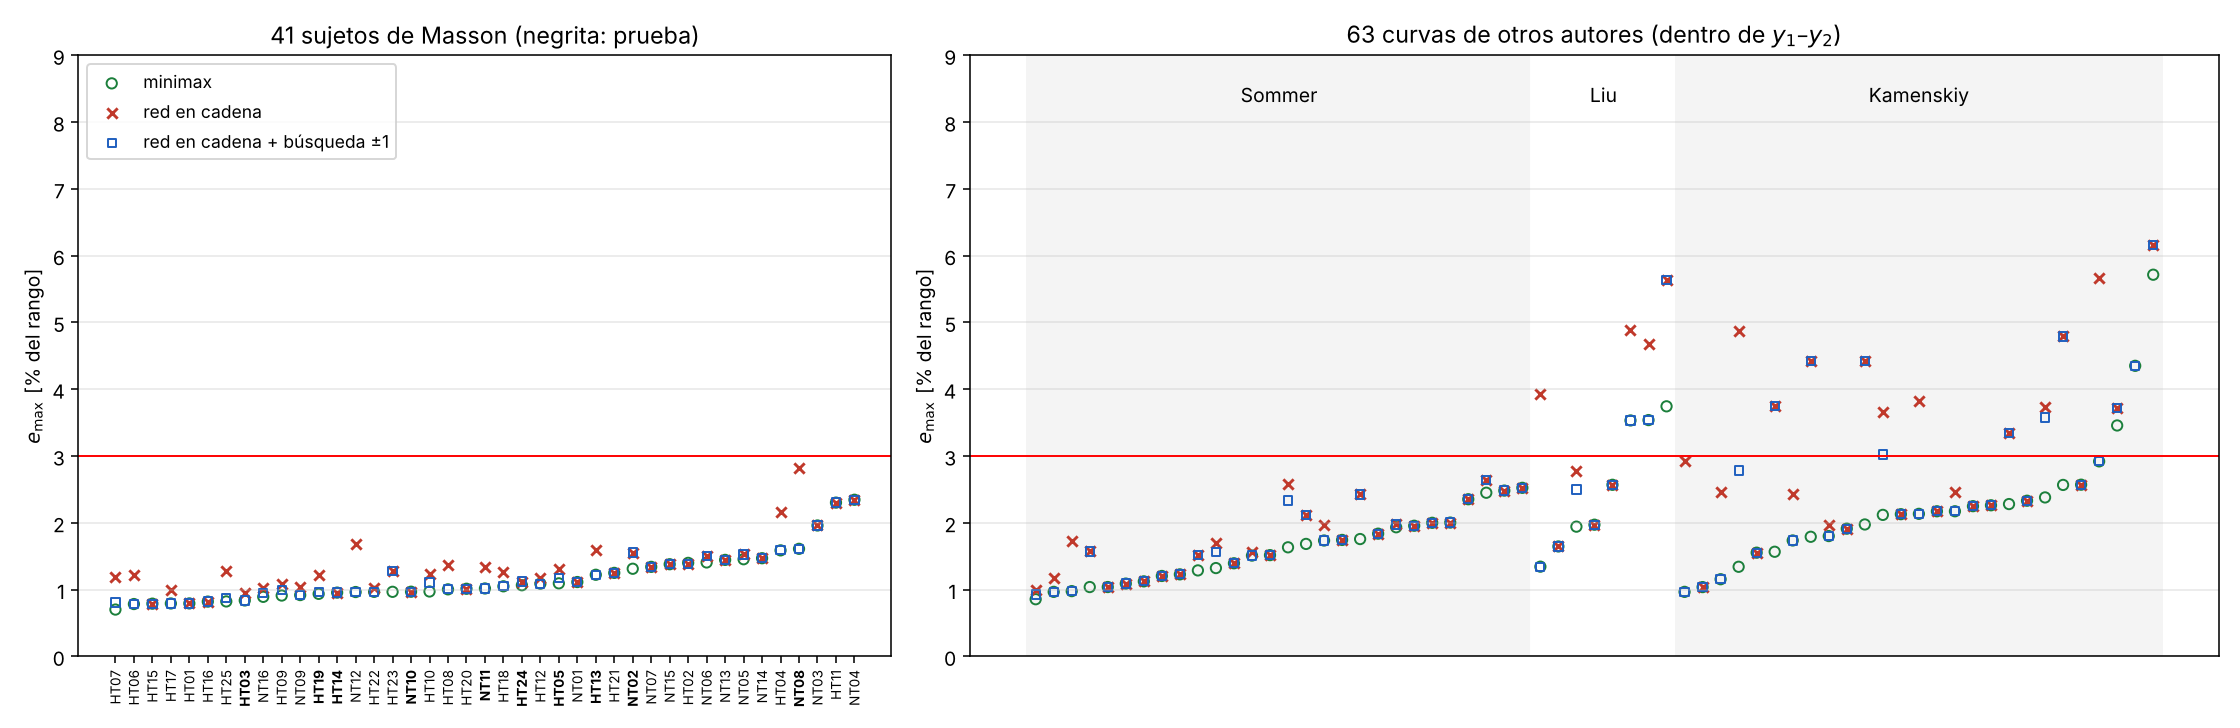
\includegraphics[width=0.9\textwidth]{v58_emax_es.png}
\caption{Peor error de cada curva con láminas enteras, 6 materiales: minimax (círculos), red en cadena (cruces) y red con revisión de $\pm1$ (cuadrados). Izquierda: los 41 sujetos (en negrita, los de prueba). Derecha: las 63 curvas de otros estudios. Línea roja: meta de 3\,\%.}\label{fig:emax}\end{figure}

%=====================================================================
\section{Cómo se usa la herramienta}
\begin{caja}{Procedimiento para una curva nueva $\sigma_{\theta\theta}(\lambda_\theta)$}
\begin{enumerate}[label=\arabic*.]
\item \textbf{Llevar la curva al dominio de diseño}: $\lambda_\theta$ entre 1,02 y 1,16, en 999 puntos. Una curva con otro tramo de estiramiento se lleva a ese intervalo con un cambio afín de $\lambda$, sin tocar las tensiones.
\item \textbf{Verificar que esté dentro del dominio de validez}: que tenga forma de J (que admita una aproximación no negativa con rectas truncadas~\cite{lawson}) y que quede entera dentro de la franja $y_1$--$y_2$.
\item \textbf{Evaluar la red}: 6 evaluaciones en cadena dan las láminas de cada material.
\item \textbf{Revisar $\pm1$ lámina} y quedarse con la combinación de menor $e_{\max}$.
\item \textbf{Comprobar} $e_{\max}\le3$\,\% contra la curva original. Si la curva no cumple el paso 2, la red no se usa y se resuelve el minimax~\eqref{eq:minimax}.
\end{enumerate}
El resultado es una representación de la curva con a lo sumo 6 materiales:
\[
\sigma_{\theta\theta}(\lambda_\theta)\approx\sum_{j=1}^{6}z_j\,S_j\,\max(0,\ \lambda_\theta-k_j),
\]
con $k_j$ y $S_j$ fijos (Tabla~\ref{tab:bases}) y $z_j$ enteros de 0 a 20.
\end{caja}

%=====================================================================
\section{Alcances y límites}
\begin{itemize}
\item \textbf{Qué se representa.} La respuesta circunferencial $\sigma_{\theta\theta}(\lambda_\theta)$ del tejido, en el borde media--adventicia y con el estiramiento axial fijo. No es una ley constitutiva tridimensional ni anisótropa: para usarla en un modelo de pared con interacción fluido--estructura habría que extenderla. Su forma (rectas truncadas que se suman) es, en cambio, muy simple de implementar.
\item \textbf{Dónde vale la red.} Solo dentro de la franja $y_1$--$y_2$ de la población de carótidas con que se entrenó. Fuera de ella el resultado no está garantizado y se usa el minimax. Otra población de arterias requiere otra franja y otro entrenamiento; el procedimiento es el mismo.
\item \textbf{El techo de las láminas enteras.} En curvas de muy poco recorrido de tensión, la división en 20 láminas por material no alcanza para la meta, ni con el minimax. Con cantidades reales cumplen todas: el límite lo pone la fabricación, no la base ni la red.
\item \textbf{Qué falta para un injerto.} Pasar de la curva del material a la curva presión--diámetro de un tubo requiere la geometría de la pared, y en la carótida la pared es gruesa: ese segundo nivel queda fuera de este resumen. Tampoco hay todavía validación experimental de un injerto fabricado.
\end{itemize}

\section{Conclusión}
Una base de materiales tipo fibra, elegida una vez para toda la población con criterios de precisión, estabilidad y fabricación, reproduce la curva tensión--estiramiento en J de las 41 carótidas de Masson et al.\ con láminas enteras y un peor error de 3\,\% o menos. El diseño minimax da el mejor diseño entero que existe, y con él se entrena una red neuronal que da las láminas de una curva nueva en una evaluación. Con una revisión de $\pm1$ lámina, la red cumple la meta en los 10 sujetos de prueba y en 50 de 63 curvas de otros estudios, el 93\,\% de lo alcanzable con láminas enteras, sin resolver ninguna optimización. Para un trabajo interdisciplinario, la herramienta ofrece una representación compacta y fabricable de la respuesta de cada arteria, obtenida al instante dentro de un dominio de validez declarado.


\begin{thebibliography}{99}\footnotesize\setlength{\itemsep}{0pt}
\bibitem{tf} Abadi, M., et al. (2016). TensorFlow: a system for large-scale machine learning. \emph{Proc. 12th USENIX OSDI}, 265--283. \url{https://www.usenix.org/conference/osdi16/technical-sessions/presentation/abadi}
\bibitem{bengiolodi} Bengio, Y., Lodi, A., Prouvost, A. (2021). Machine learning for combinatorial optimization: a methodological tour d'horizon. \emph{Eur. J. Oper. Res.} 290, 405--421. \href{https://doi.org/10.1016/j.ejor.2020.07.063}{doi:10.1016/j.ejor.2020.07.063}
\bibitem{cao} Cao, W., Mirjalili, V., Raschka, S. (2020). Rank consistent ordinal regression for neural networks with application to age estimation. \emph{Pattern Recognit. Lett.} \href{https://doi.org/10.1016/j.patrec.2020.11.008}{doi:10.1016/j.patrec.2020.11.008}
\bibitem{cheney} Cheney, E.\,W. (1966). \emph{Introduction to Approximation Theory}. McGraw-Hill.
\bibitem{cybenko} Cybenko, G. (1989). Approximation by superpositions of a sigmoidal function. \emph{Math. Control Signals Syst.} 2, 303--314. \href{https://doi.org/10.1007/BF02551274}{doi:10.1007/BF02551274}
\bibitem{dembczynski} Dembczy\'nski, K., Cheng, W., Hüllermeier, E. (2010). Bayes optimal multilabel classification via probabilistic classifier chains. En \emph{Proc. 27th Int. Conf. Machine Learning (ICML)}. \url{https://mlanthology.org/icml/2010/dembczynski2010icml-bayes}
\bibitem{ding} Ding, X., Sha, D., Sun, K., Fan, Y. (2025). Biomechanical insights into the development and optimization of small-diameter vascular grafts. \emph{Acta Biomater.} \href{https://doi.org/10.1016/j.actbio.2025.04.028}{doi:10.1016/j.actbio.2025.04.028}.
\bibitem{frankhall} Frank, E., Hall, M. (2001). A simple approach to ordinal classification. En \emph{Machine Learning: ECML 2001}, LNCS 2167. \href{https://doi.org/10.1007/3-540-44795-4_13}{doi:10.1007/3-540-44795-4\_13}
\bibitem{golub} Golub, G.\,H., Van Loan, C.\,F. (2013). \emph{Matrix Computations}, 4.ª ed. Johns Hopkins University Press.
\bibitem{harrison} Harrison, S., Tamimi, E., Uhlorn, J., Leach, T., Vande Geest, J.\,P. (2016). Computationally optimizing the compliance of a biopolymer based tissue engineered vascular graft. \emph{J. Biomech. Eng.} 138(1), 014505. \href{https://doi.org/10.1115/1.4032060}{doi:10.1115/1.4032060}
\bibitem{holzapfel} Holzapfel, G.\,A., Gasser, T.\,C., Ogden, R.\,W. (2000). A new constitutive framework for arterial wall mechanics and a comparative study of material models. \emph{J. Elasticity} 61, 1--48. \href{https://doi.org/10.1023/A:1010835316564}{doi:10.1023/A:1010835316564}
\bibitem{hornik} Hornik, K. (1991). Approximation capabilities of multilayer feedforward networks. \emph{Neural Networks} 4, 251--257. \href{https://doi.org/10.1016/0893-6080(91)90009-T}{doi:10.1016/0893-6080(91)90009-T}
\bibitem{highs} Huangfu, Q., Hall, J.\,A.\,J. (2018). Parallelizing the dual revised simplex method. \emph{Math. Program. Comput.} 10, 119--142. \href{https://doi.org/10.1007/s12532-017-0130-5}{doi:10.1007/s12532-017-0130-5}
\bibitem{humphrey} Humphrey, J.\,D. (2002). \emph{Cardiovascular Solid Mechanics: Cells, Tissues, and Organs}. Springer.
\bibitem{adam} Kingma, D.\,P., Ba, J. (2015). Adam: a method for stochastic optimization. \emph{Proc. ICLR}. \url{https://arxiv.org/abs/1412.6980}
\bibitem{lawson} Lawson, C.\,L., Hanson, R.\,J. (1995). \emph{Solving Least Squares Problems}. SIAM.
\bibitem{kamenskiy} Kamenskiy, A.\,V., Dzenis, Y.\,A., MacTaggart, J.\,N., Lynch, T.\,G., Jaffar Kazmi, S.\,A., Pipinos, I.\,I. (2012). Nonlinear mechanical behavior of the human common, external, and internal carotid arteries in vivo. \emph{J. Surg. Res.} 176(1), 329--336. \href{https://doi.org/10.1016/j.jss.2011.09.058}{doi:10.1016/j.jss.2011.09.058}
\bibitem{lilin} Li, L., Lin, H.-T. (2007). Ordinal regression by extended binary classification. \emph{Advances in Neural Information Processing Systems} 19. \url{https://proceedings.neurips.cc/paper/2006/hash/019f8b946a256d9357eadc5ace2c8678-Abstract.html}
\bibitem{linka} Linka, K., Kuhl, E. (2023). A new family of constitutive artificial neural networks towards automated model discovery. \emph{Comput. Methods Appl. Mech. Eng.} 403, 115731. \href{https://doi.org/10.1016/j.cma.2022.115731}{doi:10.1016/j.cma.2022.115731}
\bibitem{liu} Liu, H., et al. (2012). Using in vivo Cine and 3D multi-contrast MRI to determine human atherosclerotic carotid artery material properties and circumferential shrinkage rate and their impact on stress/strain predictions. \emph{J. Biomech. Eng.} 134, 011008. \href{https://doi.org/10.1115/1.4005685}{doi:10.1115/1.4005685}
\bibitem{liuml} Liu, M., Liang, L., Sun, W. (2019). Estimation of in vivo constitutive parameters of the aortic wall using a machine learning approach. \emph{Comput. Methods Appl. Mech. Eng.} 347, 201--217. \href{https://doi.org/10.1016/j.cma.2018.12.030}{doi:10.1016/j.cma.2018.12.030}
\bibitem{masson} Masson, I., Beaussier, H., Boutouyrie, P., Laurent, S., Humphrey, J.\,D., Zidi, M. (2011). Carotid artery mechanical properties and stresses quantified using in vivo data from normotensive and hypertensive humans. \emph{Biomech. Model. Mechanobiol.} 10(6), 867--882. \href{https://doi.org/10.1007/s10237-010-0279-6}{doi:10.1007/s10237-010-0279-6}
\bibitem{nair} Nair, V., Bartunov, S., Gimeno, F., et al. (2020). Solving mixed integer programs using neural networks. arXiv:2012.13349. \url{https://arxiv.org/abs/2012.13349}
\bibitem{nelder} Nelder, J.\,A., Mead, R. (1965). A simplex method for function minimization. \emph{Computer J.} 7(4), 308--313. \href{https://doi.org/10.1093/comjnl/7.4.308}{doi:10.1093/comjnl/7.4.308}
\bibitem{penrose} Penrose, R. (1955). A generalized inverse for matrices. \emph{Math. Proc. Cambridge Philos. Soc.} 51(3), 406--413. \href{https://doi.org/10.1017/S0305004100030401}{doi:10.1017/S0305004100030401}
\bibitem{read11} Read, J., Pfahringer, B., Holmes, G., Frank, E. (2011). Classifier chains for multi-label classification. \emph{Machine Learning} 85, 333--359. \href{https://doi.org/10.1007/s10994-011-5256-5}{doi:10.1007/s10994-011-5256-5}
\bibitem{rockafellar} Rockafellar, R.\,T., Uryasev, S. (2000). Optimization of conditional value-at-risk. \emph{J. Risk} 2(3), 21--41. \href{https://doi.org/10.21314/JOR.2000.038}{doi:10.21314/JOR.2000.038}
\bibitem{rovas23} Rovas, G., Bikia, V., Stergiopulos, N. (2023). Design and computational optimization of compliance-matching aortic grafts. \emph{Front. Bioeng. Biotechnol.} 11, 1179174. \href{https://doi.org/10.3389/fbioe.2023.1179174}{doi:10.3389/fbioe.2023.1179174}
\bibitem{sommer} Sommer, G., Holzapfel, G.\,A. (2012). 3D constitutive modeling of the biaxial mechanical response of intact and layer-dissected human carotid arteries. \emph{J. Mech. Behav. Biomed. Mater.} 5, 116--128. \url{https://www.sciencedirect.com/science/article/pii/S1751616111002177}
\bibitem{storn} Storn, R., Price, K. (1997). Differential evolution: a simple and efficient heuristic for global optimization over continuous spaces. \emph{J. Global Optim.} 11, 341--359. \href{https://doi.org/10.1023/A:1008202821328}{doi:10.1023/A:1008202821328}
\bibitem{tamimi} Tamimi, E.\,A., Ardila, D.\,C., Ensley, B.\,D., Kellar, R.\,S., Vande Geest, J.\,P. (2019). Computationally optimizing the compliance of multilayered biomimetic tissue engineered vascular grafts. \emph{J. Biomech. Eng.} 141(6), 061003. \href{https://doi.org/10.1115/1.4042902}{doi:10.1115/1.4042902}
\bibitem{trefethen} Trefethen, L.\,N., Bau, D. (1997). \emph{Numerical Linear Algebra}. SIAM.
\bibitem{utrera} Utrera, A., Navarrete, \'A., Bezmalinovic, A., Bertoglio, C., Celentano, D.\,J., García-Herrera, C. (2026). A deep neural network surrogate for fast mechanical parameter identification using the ring tensile test. \emph{Mater. Des.} 263, 115660. \href{https://doi.org/10.1016/j.matdes.2026.115660}{doi:10.1016/j.matdes.2026.115660}
\bibitem{vervenne} Vervenne, T., Peirlinck, M., Famaey, N., Kuhl, E. (2025). Constitutive neural networks for main pulmonary arteries: discovering the undiscovered. \emph{Biomech. Model. Mechanobiol.} 24(2), 615--634. \href{https://doi.org/10.1007/s10237-025-01930-1}{doi:10.1007/s10237-025-01930-1}
\end{thebibliography}
\end{document}
